\documentclass[oneside]{VUMIFPSkursinis}
\usepackage{algorithmicx}
\usepackage{algorithm}
\usepackage{algpseudocode}
\usepackage{amsfonts}
\usepackage{float}
\usepackage{amsmath}
\usepackage{bm}
\usepackage{caption}
\usepackage{color}
\usepackage{float}
\usepackage{graphicx}
\usepackage{listings}
\usepackage{subfig}
\usepackage{tabularx}
\usepackage{wrapfig}
\newcolumntype{P}[1]{>{\centering\arraybackslash}p{#1}}
\usepackage[%  
    colorlinks=true,
    linkcolor=black
]{hyperref}
\university{Vilniaus universitetas}
\faculty{Matematikos ir informatikos fakultetas}
\department{Programų sistemų katedra}
\papertype{Laboratorinis darbas III}
\title{Automatinė ūkio valdymo sistema}
\titleineng{Automatic Farm Management System}
\status{2 kurso 3 grupės studentai}
\author{Matas Savickis}
\secondauthor{Justas Tvarijonas}  
\thirdauthor{Greta Pyrantaitė}   
\fourthauthor{Rytautas Kvašinskas}
\supervisor{Karolis Petrauskas, Doc., Dr.}
\date{Vilnius – \the\year}


\bibliography{bibliografija}

\begin{document}
\maketitle
\tableofcontents


\section{Įvadas}
Pasaulyje technologijos vystosi labai sparčiai. Prognozuojama, kad ateityje robotizacija pakeis žmonių darbo jėgą ir žmonių darbo jėga bus nebereikalinga. Kol kas pasaulio ir Lietuvos ūkio sektoriuje robotizacija vykdoma minimaliai. Mūsų kuriama sistema siekia įnešti šią ūkio automatizaciją į Lietuvos rinką. Sistemos tikslas automatizuoti kuo daugiau ūkio veiklų. Šio laboratorinio darbo tikslas atlikti verslo analizę: atlikti išorinę ir vidinę procesų analizę, atlikti SWOT analizę, sukurti verslo vystymo strategiją ir išsiaiškinti, ar turint dabartinę rinkos, technologijų ir žinių situaciją, sistemos kūrimas ir implementavimas pasiteisintų kaip verslo planas.
\section{Verslo sritis}
	Automatinė ūkio valdymo sistemos sritis yra žemės ūkio technologijų automatizavimas, robotizavimas ir informacijos apie ūkį pateikimas. Sistema apima ūkio valdymo programinės įrangos kūrimą, automatinių sistemų įgyvendinimą, plėtojimą ir palaikymą. Į mūsų sistemos ribas neįeina vartotojo daromi verslo sprendimai bei ūkio vystymo strateginiai sprendimai. Sistemos kūrėjai neatsako už vartotojo pelno praradimą, bankrotą bei visas kitas su finansais susijusias sritis. Kūrėjai taip pat neatsako už padarytą žalą netinkamai naudojantis sistema.   

\section{Išorinė analizė}
	\subsection{Black Box analizė}
\begin{figure}[H]
		\centering	
	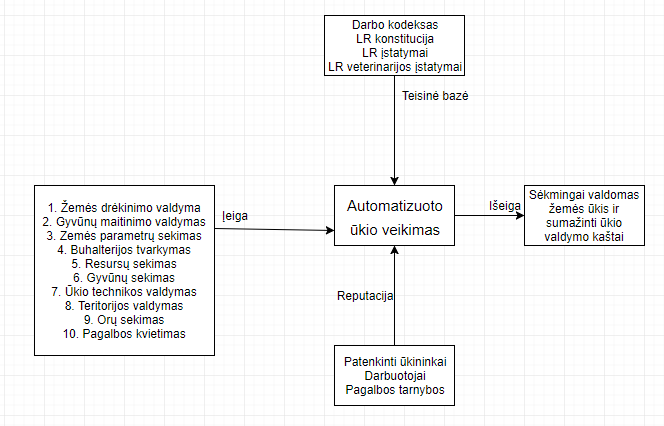
\includegraphics[width=18cm,height=20cm,keepaspectratio]{BlackBox.png}
	\caption{BlackBox diagrama}
	\label{fig:BlackBox}
\end{figure}
	\begin{itemize}
		\item{Įeiga: }
		\begin{itemize}
			\item{1. Žemės drėkinimo valdymas - vartotojas pasirenka žemės drėkinimo funkciją rankiniu arba automatiniu būdu taip užtikrindamas optimalų žemės parametrų palaikymą}
			\item{2. Gyvūnų maitinimo valdymas - vartotojas pasirenka gyvūnų maitinimą automatiniu arba rankiniu būdu taip užtikrindamas greitą, efektyvų ir humanišką gyvūnų rūpinimąsi net ir tuo atveju, kai nepavyksta pasiekti gyvūnų laiku dėl iškilusių kliūčių}
			\item{3. Žemės parametrų sekimas - vartotojui suteikiama galimybė stebėti įvairius žemės parametrus ir užtikrinti reikiamą dirvos priežiūrą ir sveikatą}
			\item{4. Buhalterijos tvarkymas - vartotojui suteikiama galimybė tvarkyti savo buhaleterinius reikalus paprastu ir suprantamu interfeisu}
			\item{5. Resursų sekimas - vartotojas turi galimybę sekti savo turimus resursus, jų rinkos kainą, ir užtikrinti maksimalų pardavimo pelną}
			\item{6. Gyvūnų sekimas - sistema užtikrina galimybę sekti kiekvieną individualų gyvūną ir pabegimo atveju jį nesunkiai surasti}
			\item{7. Ūkio technikos valdymas - sistema leidžia vartotojui valdyti ūkio techniką nuotoliniu būdu taip išvengiant žmogiškos klaidos ir taip padarant visą darbą efektyvesniu}
			\item{8. Teritorijos valdymas - sistemoje vartotojas gali žymėti savo teritoriją sutariniais ženklais, taip palengvindamas navigaciją po teritoriją}
			\item{9. Orų sekimas - sistema pateikia vartotojui orų prognozes, kurios padėtų vartotojui valdyti savo ūkį ir atsižvelgti į gamtos veiksnius}
			\item{10. Pagalbos iškvietimas - sistema suteikia galimybę išsikviesti pagalbos tarnybas ištikus nelaimingam atsitikimui.}
		\end{itemize}
		\item{Išeiga:}
		\begin{itemize}
			\item{Sistema užtikriną automatizuotą ūkio procesų valdymą, sumažina žmogaus įsikišimą į ūkio procesų valdymą, taip sumažindama žmogiško faktoriaus klaidas. Potencialiai sistema sumažina darbuotojų poreikį, kas sumažina reikalingus finansus samdyti darbuotojams bei taisyti jų padarytas klaidas}
		\end{itemize}
		\item{Teisinė bazė: }
		\begin{itemize}
			\item{Kuriant ir įgyvendinant sistemą privaloma atsižvelgti į Lietuvos Respublikos konstituciją, įstatymus bei darbo kodeksą. Jautrausia vieta teisiškai yra gyvūnų priežiūra. Šioje vietoje svarbu atsižvelgti į Lietuvos Respublikos veterinarijos įstatymus kuriant automatizuotą gyvūnų maitinimą, kad nebūtų pažeistos gyvūnų teisės }
		\end{itemize}
		\item{Reputacija: }
		\begin{itemize}
			\item{Sienkiant paversti Automatinę ūkio valdymo sistemą populiariu variantu Lietuvos ūkininkams būtina užtikrinti gerą mūsų įmonės bei sistemos reputaciją. Gerai veikianti sistema turėtų padaryti ūkininkus laimingais, kas skleistų gerą reputaciją apie mūsų sistemą ir padėtų didinti vartotojų bazę. }
		\end{itemize}
	\end{itemize}
	
	

	\subsection{Tiekimo grandinė}
	\begin{itemize}
\item Diagramoje (1 pav.) pavaizduoti pagrindiniai tiekėjai bei pirkėjai, su kuriais bendrauja mūsų nagrinėjamos srities atstovai.
		\begin{figure}[H]
		\centering	
	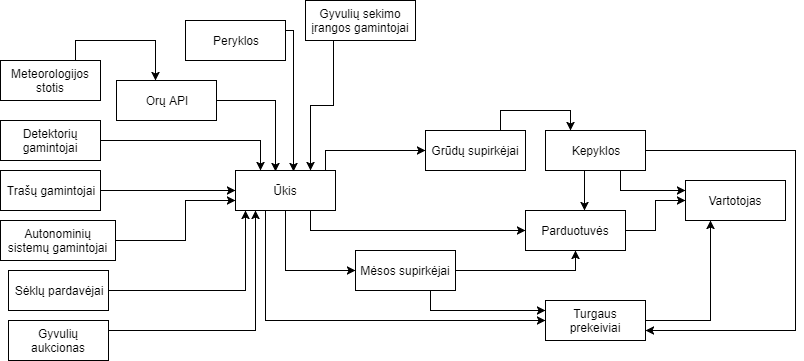
\includegraphics[width=18cm,height=20cm,keepaspectratio]{supplyChain.png}
	\caption{Tiekimo grandinė}
	\label{fig:supplyChain}
\end{figure}
\end{itemize}
\subsubsection{Pirkėjų apibrėžimas}
Kaip pagrindinius ūkio sukuriamos produkcijos pirkėjus galime įvardinti eilinius žmones, kadangi praktiškai visa ūkio produkcija suvartojama maisto pavidalu. Žinoma, dauguma žmonių šią produkciją perka ne tiesiai iš ūkininkų, o iš perpardavinėtojų ar perdirbėjų, kurie ūkio teikiamą produkciją paverčia į jau paruoštą vartoti produktą. Taigi, nors iš pirmo žvilgsnio atrodo, kad ūkio produkcijos pirkėjai yra perpardavinėtojai ir perdirbėjai, tikrieji pirkėjai yra tie, kurie perka galutinį produktą, kadangi visas darbas yra orientuotas į juos.
\subsubsection{Pirkėjų poreikiai}
Šioje diagramoje matome, kad ūkio atstovai savo produkciją paskirsto 4 keliais, tačiau juos galime padalinti į dvi dalis, ūkio tiekiama produkcija turgaus prekeiviams sudaro labai mažą dalį visos produkcijos, kadangi šią sritį dažniausiai pasirenka tie ūkininkai, kurie turi mažesnį kiekį produkcijos, ir jiems mažesnių kiekių pardavinėjimas nesukelia jokių problemų. Didesni ūkiai, priklausomai nuo jų sukuriamo produkto, paprastai renkasi parduotuves bei mėsos arba grūdų supirkėjus, kadangi jie pajėgūs produkciją supirkti labai dideliais kiekiais, taip palengvindami ūkio produkcijos administravimą. Iš šių subjektų, kurie bendrauja su ūkiu, kokybei didžiausius reikalavimus kelia turgaus prekeiviai bei parduotuvės atstovai, kadangi jie tiesiogiai bendrauja su vartotojais, o vartotojai visada tikisi aukščiausios kokybės produkcijos. O mėsos ir grūdų supirkėjai paprastai užsiima masiniu produkcijos perdirbimu, ko pasekoje šiek tiek prastesnės kokybės produktai jiems nesudaro didelių kliūčių pateikti vartotojui tinkamos kokybės produktą.
\subsubsection{Derybinės galimybės su tiekėjais}
Panašiai kaip ir pirkėjus, taip ir tiekėjus galime suskirstyti į dvi pagrindines grupes. Tokie tiekėjai, kaip trašų gamintojai, sėklų pardavinėtojai, meteorologai ar peryklos bei gyvulių pardavėjai neturi didelės derybinės galios, kadangi panašią ar netgi tokią pačią pasiūlą teikiančių tiekėjų yra pakankamai didelis kiekis, todėl patys ūkio atstovai gali išsirinkti jiems geriausius pasiūlymus iš daugelio pasirinkimų. Tačiau visai kita situacija su kitais tiekėjais,- tokie tiekėjai, kaip sekimo įrangos gamintojai, dar galbūt ir neturi labai didelės derybinės galios, tačiau likę tiekėjai gali teikti savo reikalavimus, kadangi ūkio atstovai nelabai turi kitų alternatyvų pagrindiniams šių tiekimo šakų atstovams, tokia tiekimo šaka kaip autonominių sistemų gamintojai turi maždaug 2-3 didesnius ir klientams patrauklesnius atstovus ir kiekvienas iš jų orientuojasi į šiek tiek kitą pusę, ko pasekoje ūkio atstovai turi rinktis iš daugiausiai dviejų tiekėjų, kurių kiekvienas neturi poreikio visomis išgalėmis siekti sutarties nuleidžiant kainas, kadangi jie tiesiog neturi rimtos konkurencijos.
	
	\subsection{5 Porterio jegų analizė}
	Šioje skiltyje pateiksime verslo procesų analizę pagal 5 Porterio jėgas ir išanalizuosime kiekvienos iš jėgų įtaką mūsų kompanijai.
	\begin{figure}[H]
		\centering	
	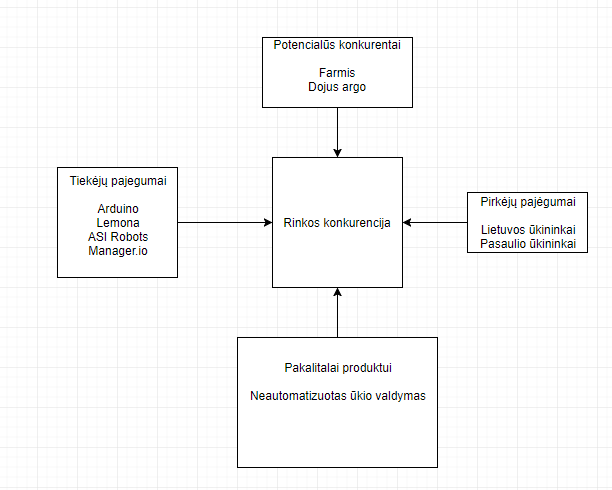
\includegraphics[width=18cm,height=20cm,keepaspectratio]{Porteris.png}
	\caption{Penkios porterio jėgos}
	\label{fig:PorterisPenki}
\end{figure}

	\begin{itemize}
		\item{Potencialūs konkurentai}
Atlikus dabartinių konkurentų Lietuvoje analizę pastebėjome, kad rinkoje egzistuoja du pagrindiniai konkurentai, užsiimantys ūkio automatizavimo verslu. Tai Farmis ir Dojus argo. Abi šios įmonės siūlo panašias įdėjas, ką bandome sukurti mes. Iš atsiliepimų ir detalesnio žvilgsnio į šias sistemas matyti, kad abi sistemos sėkmingai naudojamos Lietuvos ūkininkų ir abi šios sistemos yra pakankamai gerai išplėtotos. Pagrindinis jų trūkumas tas, kad abi šios sistemos yra gan brangios kas galbūt leistų pasinaudoti šia rinkos niša ir pasiūlyti pigesnį variantą.
		\item{Tiekėjų pajėgumai}
Mūsų sistemos įgyvendinimui labai svarbus trečios šalies tiekėjų palaikymas. Pradėjus domėtis potencialiais tiekėjais buvome maloniai nustebinti, kad visi mūsų numatyti tiekėjai turi gerą reputaciją dalių tiekimui rinkoje. Arduino yra kompanija, iš kurios pirktume mikro kontrolerius, skirtus žemės matavimams iš gyvūnų sekimui. Neradome įrasų, kad Arduino kažkada būtų turėjusi problemų su mikro kontrolerių tiekimu. Egzistuoja galimybė pirkti dideliais kiekiais, kas sumažintų kainas. Lemona yra Lietuvių elektronikos įmonė, kuri mums būtų reikalinga įvairiems smulkiems elektronikos produktams tiekti (laidams, diodams, sensoriams). ASI Robots yra įmonė, užsiimanti autonominėmis ūkio technikos sistemomis. Pagrindinė problema, kurią matome, yra tai, kad tai yra Amerikos kompanija, todėl technikos pirkimo kaštai pakiltų norint pergabenti techniką iš Amerikos į Lietuvą. Manager.io yra buhalterijos valdymo sistema. Ši sistema yra nemokama, išskyrus naudojant ją komerciniams tikslams. Tektų sudaryti sutartį dėl licensijos, bet, kadangi tai yra programinė įranga, tai net ir bankrutavus kompanijai mes vistiek galėtume naudotis jų sukurta sistema.
		\item{Pakaitalai produktui}
Atsižvelgiant į dabartinę Lietuvos ekonominę situaciją ir tai, ką pavyko perskaityti internete apie žemdirbių požiūrį į naujasias technologijas, supratome, kad pagrindinis pakaitalas mūsų sistemai būtų paprasta darbo jėga. Ūkininkai nenorėdami rizikuoti savo dabartine situacija ir papildomai investuoti į savo pelną galėtų likti prie senų ūkio valdymo modelių ir naudoti seną techniką.
		\item{Pirkėjų pajėgumai}
Įvertinus dabartinę Lietuvos ekonominę situacija priėjome išvadą, kad tokią kompleksišką sistemą įdiegti ir palaikyti kainuotų ganėtinai nemažai, todėl nemanome, kad pavyktų viską įgyvendinti taip, kaip norėjome, nes neatsirastų daug ūkininkų, norinčių investuoti didelius pinigus į šią sistema, tuo labiau, kai rinkoje jau egzistuoja panašių sistemų. Viena galima išeitis iš šios situacijos - visą sistemą padarytį pigiai, iš nebrangių dalių, bei atsisakyti kai kurių sistemos funkcionalumų.
		\item{Rinkos konkurencija}
Kaip ir minėjome, kitose skiltyse rinkoje jau egzistuoja automatinio ūkio valdymo sprendimai, tačiau jie ganėtinai brangūs. Tapti konkurencingiems rinkoje mums padėtų sistemos supaprastinimas ir jos sudarymas iš pigesnių komponentų.
		\item{Išvada} Išanalizavus dabartinę idėjos situaciją pagal 5 Porterio jėgas pastebėjome, kad pradinė mūsų idėja Lietuvos ūkininkams kainuotų per brangiai. Šios problemos sprendimas būtų atsisakyti kai kurių sistemos funkcionalumų ir padaryti pačią sistemą pigesnią. Žiūrint į tiekėjų prieinamumą nutarėme, kad  rinkoje egzistuoja tiekėjų, kurie užtikrintų reikiamų komponentų tiekimą geromis kainomis.

	\end{itemize}
	\subsection{Canvas}
	\subsubsection{Kuriama vertė}
	\begin{itemize}
		\item Procesų automatizacija
		\item Darbų paspartinimas
		\item Efektyvumo/kainos santykio padidinimas
	\end{itemize}
	\subsubsection{Klientų segmentai}
	\begin{itemize}
	\item Mažieji ūkiai, užsiimantys gyvulininkyste
	\item Didieji ūkiai, užsiimantys augalininkyste
	\item Didieji ūkiai, užsiimantys gyvulininkyste
	\end{itemize}
	\subsubsection{Komunikavimo kanalai}
	\begin{itemize}
	\item Fizinis(Pristatant techninius elementus)
	\item Mobili aplikacija
	\item Internetinė svetainė
	\item Žurnalai
	\end{itemize}
	\subsubsection{Santykių su klientais valdymas}
	\begin{itemize}
	\item Ilgalaikės sutartys
	\item Nuolaidos naujiems klientams
	\item Reklama internete
	\end{itemize}
	\subsubsection{Pajamų struktūra}
	\begin{itemize}
	\item Mėnesinis mokestis
	\item Aptarnavimo mokestis
	\end{itemize}
	\subsubsection{Resursai}
	\begin{itemize}
	\item Programuotojai
	\item Elektronikos specialistai
	\item Arduino kontroleriai
	\item Savaeigė technika
	\end{itemize}
	\subsubsection{Pagrindiniai partneriai}
	\begin{itemize}
	\item Savaeigės technikos tiekėjai(ilgalaikė sutartis dėl technikos tiekimo klientams)
	\item Ūkio žurnalai(reklama)
	\end{itemize}
	\subsubsection{Veiklos}
	\begin{itemize}
	\item Detektorių prijungimas prie sistemos
	\item Savaeigės technikos susiejimas su sistema
	\item įrangos pristatymas užsakovui
	\end{itemize}
	\subsubsection{Kaštų struktūra}
	\begin{itemize}
	\item Darbuotojų algos
	\item Serverių nuoma
	\item Reklamos kaina
	\end{itemize}
	
\subsection{Įverčiai}
\begin{figure}[H]
		\centering	
	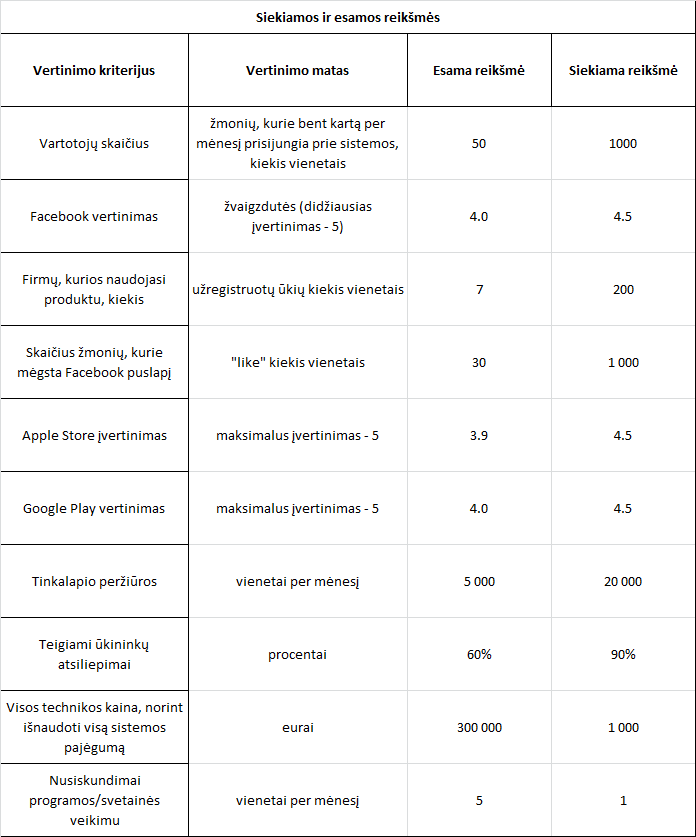
\includegraphics[width=18cm,height=20cm,keepaspectratio]{iverciai.png}
	\caption{Siekiamos ir esamos reikšmės}
	\label{fig:Iverciai}
\end{figure}
Šios metrikos padės gaudytis dabartinėje situacijoje ir geriau matyti siekiamus tiklus. Ūkių Lietuvoje nėra tiek ir daug, dauguma jų nėra pakankamai dideli kad galimai susidomėtų mūsų siūlomais funkcionalumais ir naujausiomis technologijomis. Nepaisant to, verta vis peržiūrėti šias metrikas, kad matytųsi, ar judame tinkama linkme, taip pat lengviau nustatyti mūsų sistemos efektyvumą. 
Iš įvertinimų socialiniuose tinluose, Google Play ir Apple parduotuvėse nesunku matyti, kad programai dar yra daug vietos tobulėjimui. Galimos problemos ir ką būtų galima keisti ir gerinti:
\begin{itemize}
\item Pirma problema -  kadangi mūsų sistema daug aprėpianti, inovatyvi ir priklausanti nuo naujausių technoligijų bei inovatyvumo, norint pasinaudoti visomis funkcijomis ir įdiegti pilną sistemą, kainos susidaro labai nemažos. Galima net iki 400 tūkst. eurų. Žinant, kad taikomės į negausią publiką, tokios sumos nerealios ir reikėtų jas stipriai mažinti. Galimai reikėtų mažinti funkcijų kiekį ar bent labiau susikoncentruoti į labiau prieinamas paslaugas ir mažesnius, nemilijoninius ūkius.
\item Mažokas programėlės įvertinimas ir gana didelis nusiskundimų kiekis, iš to galime spręsti, kad programinę sistemą reikia tobulinti, gerinti vartotojo sąsają, programos veikimas turėtų būti sklandesnis ir aiškesnis.
\item Maži populairumo rodikliai - reikia skirti dėmesio reklamai, žodžio skleidimui apie produktą.
\item Kadangi ūkininkai yra pagrindiniai vartotojai, o jų atsiliepimai nėra puikūs, reikia geriau išsiaiškinti, kaip padaryti sistemą jiem patrauklesnia. Pirmiausia, žinoma, reikia gerinti jau aiškias pateikimo ir kainos problemas, o po to galimai atlikti ūkininkų apklausą, kaip padaryti mūsų projektą geresniu, ko jiem labiausiai reikia iš tokio tipo sistemų ir kokios ūkio valdymo problemos jiem aktualiausios.
\end{itemize}
	
	
	
\section{Vidinė dalykinės srities analizė}
	\subsection{Vertės grandinė}
Šia skyriuje apžvelgsime kiekvieną punktą įmonės vertės grandinėje.
\begin{figure}[H]
		\centering	
	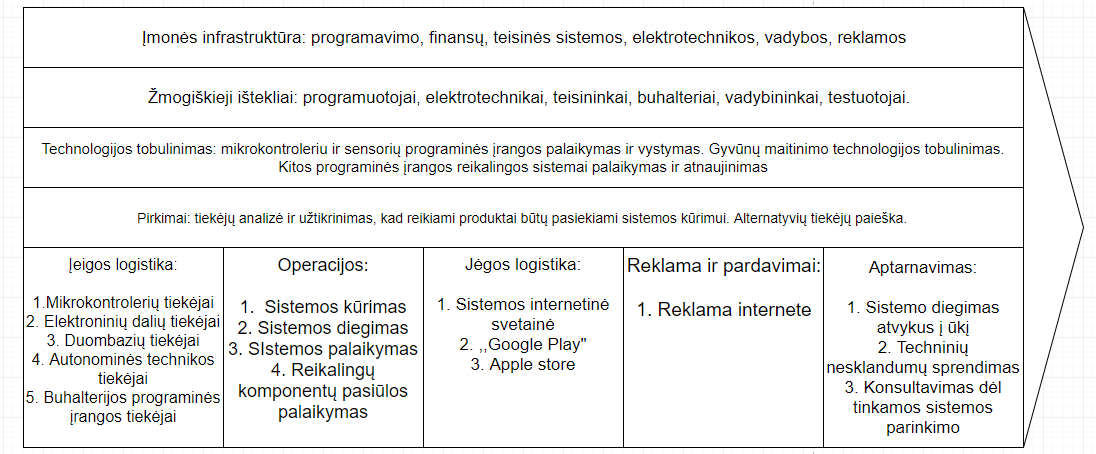
\includegraphics[width=18cm,height=20cm,keepaspectratio]{ValueChain.png}
	\caption{Vertės grandinė}
	\label{fig:VertėsGrandinė}
\end{figure}

	\begin{itemize}
		\item{Įmonės infrastruktūra: programavimo sektorius būtų atsakingas už programinės įrangos kūrimą ir plėtojimą. Finansų skyrius atsakingas už įmonės finansinę apskaitą. Teisinės sistemos skyrius atsakingas už iškilusius teisinius nesklandumus tiek su žmogiškaisiais ištekliais, tiek veterinarijos klausimais. Elektrotechnikos skyrius atsakingas už mikrokontrolerių panaudojimą, diegimą ir bendros sistemos plėtojimą. Vadybos skyrius atsakingas už žmogiškųjų išteklių valdymą. Reklamos skyriaus paskirtis - platinti informaciją apie įmonės veiklą }
		\item{Žmogiškieji ištekliai: programuotojai, testuotojai ir elektrotechnikai bus atsakingi už sklandų sistemos veikimą. Teisininkai, buhalteriai ir vadybininkai bus atsakingi už vidinių įmonės procesų palaikymą. }
		\item{Technologijos tobulinimas: sukūrus funkcionuojantį produktą įmonė ir toliau sieks optimizuoti sukurtą sistemą ir plėtoti jos panaudojimą }
		\item{Pirkimai: Bus atlikta išsami tiekėjų analizė ir išanalizuotos alternatyvos, ką tektų daryti jeigu nebebūtų įmanoma gauti prekių iš vieno iš tiekėjų.}
		\item{Įeigos logistika: Pagrindiniai komponentai reikalingi sistemai funkcionuoti yra mikro kontroleris su kita elektronika, autonominė autotechnika, duombazė ir buhalterijos aplikacija.}
		\item{Operacijos: įmonė bus atsakinga už sistemos plėtojimą, diegimą naujiems klientams, bei reikiamų komponentų pasiūla.}
		\item{Jėgos logistika: sistema Android vartotojams bus galima pasiekti per Google Play, iOS vartotojams per Apple Store, o norintiems dirbti kompiuteriu - su sukurta svetaine.}
		\item{Reklama ir pardavimai: pagrindinis sistemos populiarinimo būdas bus reklama internete}
		\item{Aptarnavimas: įmonė įsipareigoja įdiegti sistemą, tvarkyti programinius sistemos sutrikimus bei suteikti konsultaciją norint plėsti sistemą }


	\end{itemize}

	
	\subsection{Tikslai}
	\section{Proceso pjūvis}
	\begin{itemize}
	\item Transporto valdymo proceso pjūvis
	\begin{figure}[H]
		\centering	
	\includegraphics[width=18cm,height=20cm,keepaspectratio]{BPMN_transportoValdymas.png}
	\caption{BPMN transporto valdymo diagrama}
	\label{fig:BPMN_transportoValdymas}
\end{figure}
\end{itemize}
Šioje diagramoje matome, kaip bendrauja *(taisant gramatika įrašyti) vykstant transporto priemonės valdymo procesui, iš jos matome, kad vartotojui atliekant šį procesą jis siunčia sistemai pranešimus, kad ji atliktu tam tikrus patikrinimus.
	\begin{itemize}
	\item Parametrų sekimo proceso pjūvis
	\begin{figure}[H]
		\centering	
	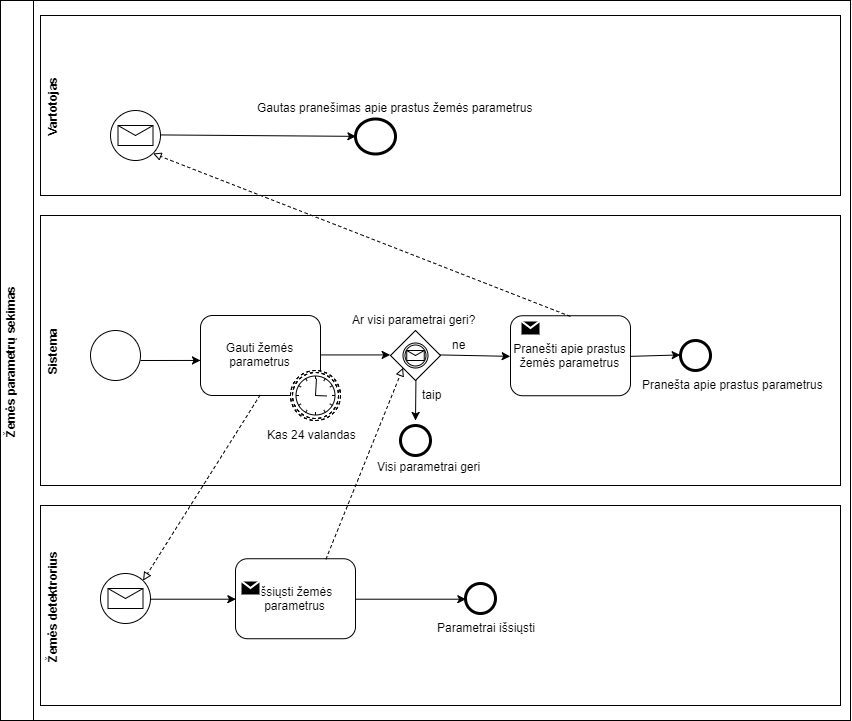
\includegraphics[width=18cm,height=20cm,keepaspectratio]{BPMN_ParametruSekimas.png}
	\caption{BPMN parametrų sekimo diagrama}
	\label{fig:BPMN_ParametruSekimas}
\end{figure}
Šioje diagramoje matome, kad sistema kas 24h automatiškai patikrina žemės parametrus ir randa akivaizdžių jų suprastėjimų apie juos praneša vartotojui, kuris juo vėliau gali sutvarkyti.
\end{itemize}
	\subsection{Veiklos principai}
	\subsection{Rodikliai}
\section{Analizės rezultatai, apibendrinimas}
	\subsection{Stiprybės}
	\begin{itemize}
	\item Sistema sukurta pagal principą, kad galėtų prisitaikyti prie kiekvienos ūkininko užgaidos, atlieka daug funkcijų.
	\item Sėkmingai įvykdžius ūkio automatizavimą galima sumažinti darbuotojų skaičių.
	\item Panaudojamos naujausios technologijos.
	\item Ir dideli, ir maži ūkiai gali naudotis programa ir ja palengvinti savo ūkio valdymą.
	\item Kadangi sistema inovatyvi, turima tam tikra persvara prieš konkurentus.
	\end{itemize}
	\subsection{Silpnybės}
	\begin{itemize}
	\item Didelė įgyvendinimo kaina.
	\item Sistema labai priklausoma nuo išorinių veiksnių, kitų įmonių, tiekėjų ir finansavimo.
	\item Mažas paklausos ratas, mažai žmonių aktuali tokia sistema.
	\end{itemize}
	\subsection{Galimybės}
	\begin{itemize}
	\item Programai populiarėjant galimas plėtimasis į kitas Europos šalis.
	\item Galima mažinti kainas, naudoti įperkamesnias detales.
	\item Vertėtų taikytis į didesnę publiką, prisitaikyti prie įvairaus dydžio ir poreikių ūkių/sodybų.
	\end{itemize}
	\subsection{Pavojai}
	\begin{itemize}
	\item Yra nemažai konkurentų, kurie teikia kokybišką produktą ir turi realistiškesnį panaudojimą.
	\item Kadangi publika, į kurią taikomės yra labai specifiška ir negausi, nėra didelės tikimybės, kad investicijos pasiteisins ir mūsų produktas taps populiarus.
	\item Dėl mažos paklausos galimas mažas pelnas.
	\item Dėl didelių sistemos įgyvendinimo kaštų dar labiau sumažėjau paklausa.
	\item Sistema labai sudėtinga, priklausoma, labai daug niuansų, kuriuos ateityje gali būti sunku suvaldyti.
	\end{itemize}
	
\section{Vizija, misija}
\subsection{Mission}
Misija - sukurti aplikaciją, kuri leistų ūkininkams valdyti savo ūkį su kuo mažiau žmogiškosios interakcijos bei konkuruotų pasaulinėje rinkoje.
\subsection{Objectives}
Tikslai - sukurti aplikaciją, kuri valdytų ūkį su minimalia žmogaus pagalba.
Sutelkti visą informaciją, aktualią ūkio priežiūrai/valdymui, į vieną vietą.
Įtraukti į aplikaciją įvairias sistemas, kuriomis būtų galima sumažinti žmogaus indelį.
Pritaikyti programą naudojimui visoje Lietuvoje.
Sukurti patogią, patrauklią bei paprastą grafinę vartotojo sąsają.
\subsection{Strategies}
Strategijos - surinkti informaciją dėl programos turinio, sužinoti, kokia informacija ūkininkams yra esminė prižiūrint ūkį.
Išpopuliarinti sistemą tarp Lietuvos ūkininkų.
Surinkti informaciją apie tinkamą, patogią ir patrauklią grafinę vartotojo sąsają.
\subsection{Tactics}
Taktikos - surinkti informaciją dėl programos turinio, atliekant potencialių vartotojų apklausą.
Išanalizuoti panašias sistemas, įvertinti, kokia informacija yra plačiausiai naudojama jose.
Paruošti apklausą bei apklausą vykdančius darbuotojus, kurios tikslas būtų išrinkti tinkamiausią grafinę vartotojo sąsają.
Išsiaiškinti, kurie funkcionalumai yra aktualiausi vartotojams, pateikiant potencialiems vartotojams apklausas.
\section{Strateginiai tikslai}
	Mūsų pagrindinis tikslas yra padaryti, kad ūkio valdyme būtų kuo mažiau žmogaus įsikišimo. Atlikdami verslo analizę supratome, kad Lietuvos rinka yra salyginai maža, o ekonominė situacija prasta lyginant su kitomis šalimis. Todėl nutarėme, kad mūsų sistema turi būti kuo prieinamesnė ir pigesnė vartotojui, paaukojant kuo mažiau funkcionalumų. Dalis ūkininkų yra senyvi žmonės, per daug nesusipažinę su technologijomis. Taip pat Lietuvoje nėra tiek daug didelių žemės ūkių, todėl savo strategijoje turime atsižvelgti ir į mažus ūkininkus ar net žmones turinčius sodybas. Savo strategija sieksime padaryti, kad kiekvienas ūkininkas būtų kuo labiau informuotas apie savo turimą ūkį. Mūsų pagrindinės strategijos žingsniai bus:
	\begin{itemize}
		\item{Sistemos kainos mažinimas: atlikdami verslo analizę supratome, kad norėdami išlikti kompetetingi rinkoje turime kiek galima sumažinti sistemos kainą. Kainą mažinsime pirkėjui suteikdami galimybę rinktis mažesnį ir paprastesnį sistemos variantą.  Vietoj pilnos sistemos, kuri valdo ūkio techniką ir automatiškai šeria gyvunus, mes suteiksime galimybę pasirinkti tik žemės parametrų sekimą ir automatinį laistymą. Taip pat suteiksime vartotojams galimybę patiems įsidiegti sistemą jeigu jie nenorės mokėti už mūsų diegimo paslaugas. Toks modalumas leistų sistemą įdiegti net ir sodybose ir drastiškai sumažintų primityvios sistemos kainą.}
		\item{Sistemos prieinamumas seniems žmonėms bei žmonėms su negalia: kurdami interfeiso dizainą atsižvelgsime į dizaino prieinamumą(accessability). Programinės įrangos interfeisas bus kontrastingų spalvų. Bus galima pakeisti sąsajos komponentų dydžius. Tai suteiks lengvesnį prieinamumą žmonėms su motorinėmis ar regos negalėmis. Suteiksime išsamius paaiškinimus kaip naudotis sistema. Vartotojui pageidaujant atvyksime įdiegti ir sukonfiguruoti sistemą}
		\item{Sistemos panaudojimas mažiems ūkiams: siekiant pritraukti kuo didesnį kiekį vartotojų savo produktą kursime ne tik didiesiems ūkininkams, bet taip pat ir sodybų savininkams, turintiems nedidelius žemės plotus. Mažų žemės plotų savininkai galės nusipirkti tik laistymo ir parametrų stebėjimo funkciją. Minimalus sistemos variantas kainuotų salyginai pigiai ir vartotojas galėtų palikti savo žemę programos priežiūroje, kuri ją laistytų.}
		\item{Informavimas apie ūkį: savo sistema sieksime ūkininką kuo labiau informuoti apie jo valdomą teritoriją, suteikti informaciją apie žemės parametrus ir pateikti rekomendacijas, ką daryti kokioje situacijoje. Sistema suteiks rekomendacijas, kada laistyti žemę, kada nuimti derlių, kokiomis trašomis tręšti žemę, kada sėti. Sistema suteiktų informacijos net ir norintiems pradėti užsiimti ūkininkavimu.}
		\item{Sistemos pritaikymas dideliems ūkiams: siekiant apimti kuo didesnį rinkos gabalą sistema bus pritaikyta ir didiesiems ūkininkams. Vartotojui bus suteiktos galimybės laistyti didelius žemės plotus, stebėti žemės parametus, sekti rinkos kainas, užsisakyti autonominę ūkio techniką bei tvarkyti buhalteriją.}
	\end{itemize}
\section{Sistemos naudojimo scenarijus}
\subsection{scenarijai}
\begin{itemize}
\item Sistemos administratorius gali būti perspėtas dėl netinkamai funkcionuojančių detektorių
\begin{figure}[H]
		\centering	
	\includegraphics[width=18cm,height=20cm,keepaspectratio]{gedimoŠalinimas.png}
	\caption{Detektoriaus gedimo šalinimo sekų diagrama}
	\label{fig:gedimoŠalinimas}
	\end{figure}
	Tam, kad sistemos administratoriui nereiktų nuolat tikrinti, ar visi žemės detektoriai tinkamai funkcionuoja, programos vartotojas turi galimybę pranešti apie jo nuomone netinkamai funkcionuojantį prietaisą. Po šio pranešimo administratorius patikrina jo pagrįstumą ir klaidos atveju pasistengia ją kuo greičiau ištaisyti.
\end{itemize}

\subsection{Sistemos teikiama nauda}

\section{Sistemos įgyvendinimo planas}
Sistemą įgyvendinsime pagal žemiau pateiktą diagramą. 
\begin{figure}[H]
		\centering	
	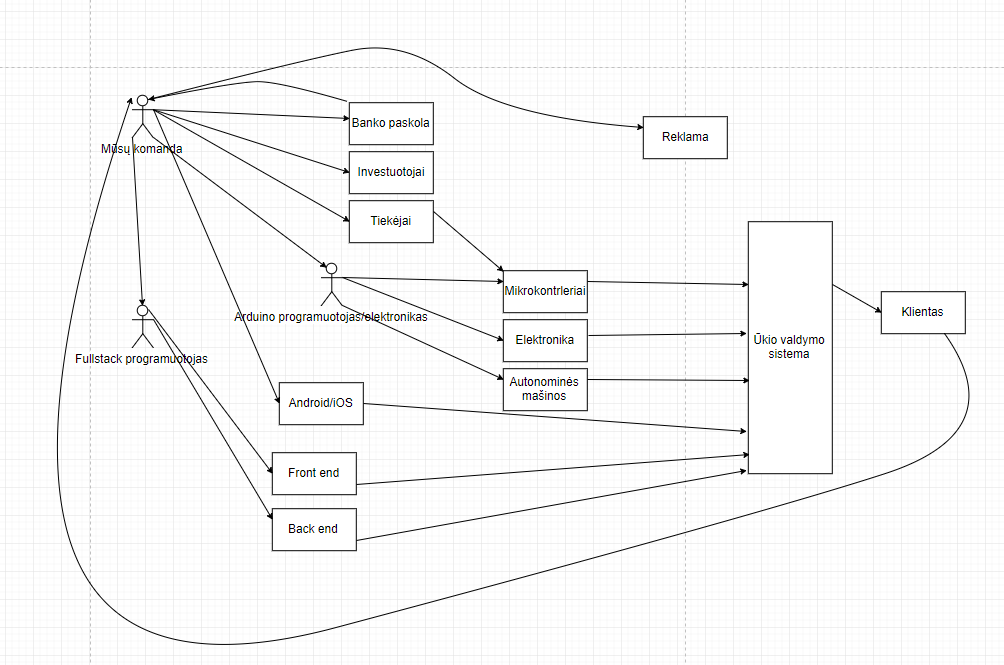
\includegraphics[width=18cm,height=20cm,keepaspectratio]{SistemosIgyvendinimas.png}
	\caption{Sistemos įgyvendinimo planas}
	\label{fig:Sistemos įgyvendinimo planas}
\end{figure}
Pirmoje sistemos įgyvendinimo fazėje mūsų komanda pasamdys du programuotojus: Fullstack programuotoją ir Arduino programuotoją/elektroniką. Fullstack programuotojas bus atsakingas už svetainės, serverių ir duombazės kūrimą bei palaikymą. Arduino programuotojas kurs sistemą, kuri valdys sensorius ir gyvūnų maitinimą. Tuo tarpu dalis mūsų komandos kurs Android/iOS aplikacijas, o kita dalis rūpinsis derėjimusi su tiekėjais, investuotojų pritraukimu ir, jeigu reikės, banko paskolos gavimu. Kai sistema artės prie parduodamo produkto mūsų komanda pradės reklamuoti mūsų sistemą suinteresuotiems pirkėjams. Paskutinioje fazėje programuotojai apjungs viską į vieną sistemą ir sistema bus pateikta pardavimui klientams. 


\section{Įgyvendinamumo analizė}
	\subsection{Operacinė analizė}
\begin{table}[htbp]
	\begin{tabularx}{1\textwidth}{ |P{7.5cm}|X| }  \hline
		Problema & Problemos pašalinimas \\ \hline
		Vartotojai nežinos šios programos & Išreklamuoti programą įvairiuose ūkininkams aktualiuose puslapiuose, bet ūkininkams aktualių televizijos laidų metu \\ \hline
		Vartotojai nemokės naudotis programa & Sistemoje įterpti naudojimo instrukciją \\ \hline
	\end{tabularx}
\end{table}
	\subsection{Techninė analizė}
Atlikę techninę analizę išgryninom idėjas, kokių techninių komponentų reikia įgyvendinti sistemą. Visas ūkio valdymas būtų vykdomas Arduino mikrokontroleriu, kurį galima nusipirkti iš nevieno tiekėjo. Kartu su kontroleriu sistemai reiktų sensorių bei laidų, kuriuos taip pat galima nesunkiai įsigyti. Sistemos veikimui užtikrinti reiktų duombazės, kurioje būtų saugoma įvairi informacija. Duombazė būtų laikoma serveryje. Autonominę techniką gautume iš ASI Robots, kartu su technika gautume ir programinę įrangą, skirtą kontroliuoti šią techniką.
	\subsection{Ekonominio įgyvendinamumo analizė}
	\begin{itemize}
		\item{Išlaidos: Savo įmonės išlaidas išskirsime į dvi kategorijas: kiek kainuos kiekviena siūloma paslauga ir kiek pinigų reikės verslui pradėti ir sistemai sukurti}
		\begin{itemize}
			Siulomos paslaugos ir jū išlaidos:
			\newline
			Mažo ūkininko paketas
			\item{Arduino mikrokontroleris 20eu}
			\item{Laidai sujungimui 20eu}
			\item{Laisrymo žarna: 60eu(priklauso nuo žemės ploto)}
			\item{Sprinkleriai: 20eu}
			\item{Sensoriai: 100eu}
			\item{Savikaina: 220eu}	
			\item{Kaina: 500eu}
			\newline
			Vidutinio ūkininko paketas(įeina viskas kas viršuje plius kas pateikta apačioje)
			\item{Automatinio maitinimo įranga: 500eu(pagal reikalinga kiekį)}
			\item{Gyvūnų sekimo iranga: 1000eu (priklauso nuo gyvūnu kiekio)}
			\item{Savikaina: 2000eu}
			\item{Kaina: 3000eu}
			\newline
			Didelio ūkininko paketas(viskas kas viršuje):
			\item{Automatizuota technika: 100000eu(priklausomi nuo technikos kiekio)}
			\item{Savikaina 140000eu}
			\item{Kaina: 150000eu}
			\newline
			Kaina yra kiek preliminariai planuojam prašyti už paslaugą
			
		\end{itemize}
		\item{Išlaidos reikalingos komandai išlaikyti:}
		\begin{itemize}
			\item{Fullstack programuotojo atlyginimas mėnesiui 2000eu}
			\item{Administratorius 500eu}
			\item{Arduino programuotojas/elektronikas 2000eu}
			\item{Serverio išlaidos: 100eu mėnesiui}
			\item{Verslo licensija: 1000eu}
			\item{Reklama mėnesiai: 500eu}
		\end{itemize}
		Įkuriant įmonė reikės susimokėti licensijos mokestį 1000eu ir realaus produkto pateiki vartotojui negalėsime dar 4 mėnesius nes reikės ją sukurti, šią kainą sumažiną tai, kad mes patys galėsime prisidėti prie sistemos kūrimo programuojant. Kas mėnesį įmonės išlaikymas mums kainuos maždaug 5500eu. Taigi praždžiai reikės maždaug 20000eu investicijos. 
		\newline
	

		
		\item{Pajamos:}
Lietuvoje yra maždaug 120000 ūkių iki 30 hektarų. Šiems ūkiams galėtume pasiūlyti savo mažo ūkininko paketa. Jeigu manysime kad pavyks 1 procentui ūkininkų parduoti mažiausią sistemos paketą gautime 300000eu pelno.Papildomai vartotojas turėtų mokėti prenumeratos mokestį už sistemos palaikyma ir gedimų šalinimą 50eu per mėnesiui. Sistema veiktų maždaug pusę metų(žiemą nereikia laistyti) už sistemos prenumeratas per metus turėtume gauti 200000eu pelno išskaičiavus taisymo kainas.
		\newline
		Lietuvoje yra 4000 ūki kurių plotas nuo 30 iki 100 hektarų. Šiem ūkininkam siūlytume vidutinį paketa. Jeigu pavyktų parduoti procentui šių ūkininkų vidutinę sistemą sistemą gautume maždaug 40000eu pelno. Už mėnesinę prenumeratą gautume 12000eu.
		\newline
		Ūkių turinčių daugiau negu 100 hektarų žemės tėra 500. Todėl manome, kad didžiausią paketą pavyktų parduoti tik vienetams. Todėl galimo pelno skaičiuoti neverta.
		
		\item{Apibendrinimas:}
		\newline
		Atlikę ekonominę analizę išsiaiškinome, kad prasmingia būtų sumažinti projekto apimtį ir tiekti mažajį ir vidutinį ūkininko paketus siekiant minimalizuoti riziką.


	\end{itemize}
	\subsection{Teisinė analizė}
Mūsų kuriamai sistemai svarbiausias teisinis klausimas - ar nebus pažeistas asmens duomenų teisinės apsaugos įstatymas. Mūsų sistemos funkcionalumas ir tikslai nepažeidžia asmens duomenų apsaugos įstatymo tikslo - “ginti žmogaus privataus gyvenimo neliečiamumo teisę tvarkant asmens duomenis”. Mūsų sistema registracijos metu neprašo jokių asmeninių duomenų. Prašome tik susisiekimui su vartotoju reikalingos informacijos bei vartotojui kuriantis paskyrą bus prašoma įvesti jo paties sugalvotą slapyvardį, kuris bus naudojamas jo identifikacijai, nuslepiant jo tapatybę.
\section{Išvados}
	Šia darbe išanalizavome mūsų verso idėją. Įvertinome vidinius ir išorius veiksnius. Analizės metu supratome, kad mūsų idėjos apimtis Lietuvai yra per didelė. Mažoje Lietuvos rinkoje nepavykų įgyvendinti autonominės ūkio technikos idėjos, nes kaštai būtų per dideli relityviai mažiems Lietuvos ūkininkams. Tačiau padarėmę išvadą, kad atitinkiamai pritaikius sistemą mažiems ūkiams ir sodyboms idėja turi šansų susilaukti dėmesio. Lietuvos rinkoje jau yra automatizuotų ūkių sprendimų, tačiau jie labiau pritaikyti dideliems ūkiam. Taikantis į sodybas ir mažus ūkius, bandant kuo labiau sumažinti sistemos kainas yra galimybė gauti pelno. Verta paminėti, kad vienas Lietuvos rinkos privalumas yra tai, kad programuotojų algos yra mažesnės negu kitos šalyje, kas sumažintų pradinę sistemos kūrimo kainą.
	
 
\section{Žodynas}
\begin{itemize}
\item ASI - kompanija, kuri teikia automatiškai valdomą transportą.
\item Automatiškai valdoma - valdymui nereikalinga žmogaus pagalba.
\item Black Box - programa, sistema ar įrenginys, į kurį galima žvelgti kaip į jo įeitį/išeitį nežinant, kaip jis iš tiesų veikia viduje.
\item Dalykinė sritis – sritis, kurioje naudojama sistema.
\item Detektorius - Arduino mikro kontroleris, skirtas ūkio sekimui.
\item Naudotojas/vartotojas - žmogus, kuris naudojasi programa.
\item Penkių Porterio jėgų modelis - nagrinėja naujų konkurentų įėjimo baimę, vartotojų (pirkėjų) perkamąją galią, tiekėjų derėjimosi galią, substitutų baimę bei konkurenciją šakoje.
\item Manager.io - buhalterijos valdymo sistema
\item SWOT - strengths, weaknesses, opportunities, ir threats santrumpa (stiprybės, silpnybės, galimybės, pavojai).
\end{itemize}

\end{document}